\documentclass{assignment}
\usepackage[utf8]{inputenc}
\usepackage[T1]{fontenc}
\usepackage{hyperref}
\usepackage{listings}

\lstset{
	inputencoding=utf8,
	literate=
	{á}{{\'a}}1
	{é}{{\'e}}1
	{í}{{\'i}}1
	{ó}{{\'o}}1
	{ú}{{\'u}}1
	{Á}{{\'A}}1
	{É}{{\'E}}1
	{Í}{{\'I}}1
	{Ó}{{\'O}}1
	{Ú}{{\'U}}1
	{ñ}{{\~n}}1
	{Ñ}{{\~N}}1
}


\lstdefinelanguage{Pseudocodigo}{
	morekeywords={
		SI, ENTONCES, SINO, FIN, MIENTRAS, HACER, PARA, DESDE, HASTA,
		FUNCIÓN, PROCEDIMIENTO, CLASE, CONSTRUCTOR, ATRIBUTOS,
		RETORNAR, ALGORITMO, CONSTANTE, NUEVO, Y, O, NO, CADA, EN
	},
	sensitive=false,
	morecomment=[l]{//},
	morestring=[b]",
}

\lstset{
	language=Pseudocodigo,
	basicstyle=\ttfamily\small,
	keywordstyle=\color{blue}\bfseries,
	commentstyle=\color{gray}\itshape,
	stringstyle=\color{orange},
	numbers=left,
	numberstyle=\tiny\color{gray},
	stepnumber=1,
	breaklines=true,
	frame=single,
	tabsize=4,
	showstringspaces=false,
}
\begin{document}
	
	\assignmentTitle{Claudio Iván Esparza Castañeda}{Luis Alberto Balam Guzmán}{./Logo.png}{Maestría en Sistemas Embebidos}{Programación y Procesamiento de Datos}{2B. Práctica de procesamiento numérico y científico con Python}
	
	\section*{Objetivo}
	Más allá de las funciones incluidas en el estándar de Python, la amplia comunidad comenzó a implementar funciones más complejas que agrupan múltiples funciones orientadas a tópicos específicos. La idea es que no se tenga que reinventar la rueda cada vez. Con este espíritu es que se crearon módulos (propiamente el equivalente de las bibliotecas o librería de otros lenguajes) como NumPy, el cual tiene funciones para manipular una arreglos, como una generalización de las listas. Permite manipular para obtener cálculos matemáticos que incluyen (sin limitarse) al álgebra lineal y la estadística.\\
	La popularidad de Numpy en forma reciente viene de su uso en análisis de datos, de la inteligencia artificial, entre otros campos. Las aplicaciones, claro, son infinitas y corresponde a uno plantearse la manera en que quisiera realizar estas tareas.\\
	En prácticas anteriores he creado funciones que he ido reciclando y ahora las junto en un módulo {\tt funciones}, y quizá de esta versión 1 pueda seguir creciendo en las prácticas sucesivas.
	Combinando los conocimientos usados en las pácticas anteriores, se combina para tener clases, listas iterables, y ahora el uso de NumPy para tener arreglos para analizar datos obtenidos con anterioridad.\\
	Este programa involucra el uso de un menú para el control del flujo. Se cuenta con validaciones para los distintos tipos de datos que se emplean en el programa, y se cuenta con una Clase "Clima" con métodos para cada etapa opción del menú.
	\section*{Pseudocódigo}
	Ya desde prácticas anteriores PSeInt estaba rebasado para plasmar estos algoritmos más complejos, aquí traté de expresarlo en lenguaje natural. Por la simpleza de python, mucho fue traducir de inglés a español.
	\subsection*{Inicialización}
	\begin{lstlisting}[caption={Inicialización}, label={lst:inicio}]
		CONSTANTE N_LECTURAS <- 10
		PROCEDIMIENTO Menu()
			IMPRIMIR "==========================="
			IMPRIMIR " Análisis de Datos Climáticos"
			IMPRIMIR "==========================="
			IMPRIMIR "1. Capturar datos"
			IMPRIMIR "2. Imprimir datos"
			IMPRIMIR "3. Calcular estadísticas"
			IMPRIMIR "4. Indexamiento y filtrado"
			IMPRIMIR "5. Álgebra lineal"
			IMPRIMIR "6. Funciones especiales"
			IMPRIMIR "7. Salir"
		FIN PROCEDIMIENTO
	\end{lstlisting}
	\subsection*{Clase Clima}
		\begin{lstlisting}[caption={Clase Clima}, label={lst:clima}]
		CLASE Clima
			ATRIBUTOS
				temperatura : Lista de Real
				humedad     : Lista de Real
				viento      : Lista de Real
			CONSTRUCTOR Clima()
				temperatura <- [ ]
				humedad     <- [ ]
				viento      <- [ ]
			FIN CONSTRUCTOR
			FUNCIÓN NoVacio(): Booleano
				RETORNAR Longitud(temperatura) > 0
			FIN FUNCIÓN
			PROCEDIMIENTO Capturar()
				IMPRIMIR "--- Capturar datos (", N_LECTURAS, " lecturas) ---"
				temperatura <- [ ]
				humedad     <- [ ]
				viento      <- [ ]		
				PARA i DESDE 1 HASTA N_LECTURAS HACER
					IMPRIMIR "-- Día ", i, " --"
					Agregar(temperatura, PedirReal("  Temperatura día " + i + ": "))
					Agregar(humedad,     PedirReal("  Humedad día "     + i + ": "))
					Agregar(viento,      PedirReal("  Viento día "      + i + ": "))
				FIN PARA
				IMPRIMIR "Datos capturados correctamente."
			FIN PROCEDIMIENTO
			PROCEDIMIENTO Imprimir()
				IMPRIMIR "--- Datos capturados ---"
				SI NO NoVacio() ENTONCES
					IMPRIMIR "No hay datos capturados todavía."
					RETORNAR
				FIN SI
				IMPRIMIR "Temperaturas: ", temperatura
				IMPRIMIR "Humedades: ", humedad
				IMPRIMIR "Vientos: ", viento
			FIN PROCEDIMIENTO
			PROCEDIMIENTO Estadisticas()
				IMPRIMIR "--- Estadísticas ---"
				SI NO NoVacio() ENTONCES
					IMPRIMIR "No hay datos capturados todavía."
					RETORNAR
				FIN SI
				variables <- [("Temperatura", temperatura), ("Humedad", humedad), ("Viento", viento)]
				PARA CADA (nombre, arreglo) EN variables HACER
					IMPRIMIR nombre, ":"
					IMPRIMIR "  Media: ", Media(arreglo)
					IMPRIMIR "  Máximo: ", Maximo(arreglo)
					IMPRIMIR "  Mínimo: ", Minimo(arreglo)
					IMPRIMIR "  Desviación estándar: ", DesviacionEstandar(arreglo)
				FIN PARA CADA
			FIN PROCEDIMIENTO
			PROCEDIMIENTO Filtrado()
				IMPRIMIR "--- Indexamiento y filtrado ---"
				SI NO NoVacio() ENTONCES
					IMPRIMIR "No hay datos capturados todavía."
					RETORNAR
				FIN SI
				promedio_temp <- Media(temperatura)
				dias_temp_alta <- [ ]
				valores_temp_alta <- [ ]
				PARA i DESDE 1 HASTA Longitud(temperatura) HACER
					SI temperatura[i] > promedio_temp ENTONCES
						Agregar(dias_temp_alta, i)
						Agregar(valores_temp_alta, temperatura[i])
					FIN SI
				FIN PARA
				IMPRIMIR "Promedio de temperatura: ", promedio_temp
				IMPRIMIR "Días con temperatura mayor al promedio: ", dias_temp_alta
				IMPRIMIR "  Valores: ", valores_temp_alta
				dias_humedad_baja <- [ ]
				valores_humedad_baja <- [ ]
				PARA i DESDE 1 HASTA Longitud(humedad) HACER
					SI humedad[i] < 40 ENTONCES
						Agregar(dias_humedad_baja, i)
						Agregar(valores_humedad_baja, humedad[i])
					FIN SI
				FIN PARA
				IMPRIMIR "Días con humedad menor a 40: ", dias_humedad_baja
				IMPRIMIR "  Valores: ", valores_humedad_baja
				dias_combo <- [ ]
				temps_combo <- [ ]
				vientos_combo <- [ ]
				PARA i DESDE 1 HASTA Longitud(temperatura) HACER
					SI temperatura[i] > 30 Y viento[i] > 20 ENTONCES
						Agregar(dias_combo, i)
						Agregar(temps_combo, temperatura[i])
						Agregar(vientos_combo, viento[i])
					FIN SI
				FIN PARA
				IMPRIMIR "Días con temperatura > 30 y viento > 20: ", dias_combo
				IMPRIMIR "  Temperaturas: ", temps_combo
				IMPRIMIR "  Vientos: ", vientos_combo
			FIN PROCEDIMIENTO
			PROCEDIMIENTO Algebra()
				IMPRIMIR "--- Álgebra lineal ---"
				SI NO NoVacio() ENTONCES
					IMPRIMIR "No hay datos capturados todavía."
					RETORNAR
				FIN SI
				temp_norm <- Normalizar(temperatura)
				hum_norm  <- Normalizar(humedad)
				vien_norm <- Normalizar(viento)
				IMPRIMIR "Vectores normalizados:"
				IMPRIMIR "  Temperatura: ", temp_norm
				IMPRIMIR "  Humedad: ", hum_norm
				IMPRIMIR "  Viento: ", vien_norm
				dot_temp_hum  <- ProductoPunto(temp_norm, hum_norm)
				dot_temp_vien <- ProductoPunto(temp_norm, vien_norm)
				IMPRIMIR "Producto punto Temperatura-Humedad: ", dot_temp_hum
				IMPRIMIR "Producto punto Temperatura-Viento: ", dot_temp_vien
				matriz <- ApilarFilas(temp_norm, hum_norm, vien_norm)
				IMPRIMIR "Matriz 3x", N_LECTURAS, " de datos normalizados:"
				IMPRIMIR matriz
				corr <- MatrizCorrelacion(matriz)
				IMPRIMIR "Matriz de correlación 3x3 (Temperatura, Humedad, Viento):"
				IMPRIMIR corr
			FIN PROCEDIMIENTO
			PROCEDIMIENTO FuncionesEspeciales()
				IMPRIMIR "--- Funciones especiales ---"
				SI NO NoVacio() ENTONCES
					IMPRIMIR "No hay datos capturados todavía."
					RETORNAR
				FIN SI
				indice_termico <- [ ]
				PARA i DESDE 1 HASTA Longitud(temperatura) HACER
					Agregar(indice_termico, temperatura[i] * Exponencial(humedad[i] / 100))
				FIN PARA
				IMPRIMIR "Índice térmico simulado (IT = temperatura * exp(humedad/100)):"
				IMPRIMIR "Primeros 5 valores: ", SubLista(indice_termico, 1, 5)
			FIN PROCEDIMIENTO	
		FIN CLASE
	\end{lstlisting}
	\subsection*{Otras funciones}
	\begin{lstlisting}[caption={Otras funciones}, label={lst:otras}]
		FUNCIÓN Normalizar(vector): Lista de Real
			norma <- RaízCuadrada(Sumatoria de vector[i]^2 PARA CADA i EN vector)
			SI norma = 0 ENTONCES
				RETORNAR vector
			FIN SI
			resultado <- [ ]
			PARA CADA valor EN vector HACER
				Agregar(resultado, valor / norma)
			FIN PARA CADA
			RETORNAR resultado
		FIN FUNCIÓN
		FUNCIÓN ProductoPunto(v1, v2): Real
			suma <- 0
			PARA i DESDE 1 HASTA Longitud(v1) HACER
				suma <- suma + v1[i] * v2[i]
			FIN PARA
			RETORNAR suma
		FIN FUNCIÓN
	\end{lstlisting}
	\subsection*{Algoritmo principal}
	\begin{lstlisting}[caption={Algoritmo principal}, label={lst:principal}]
		ALGORITMO Principal
			opcion <- 0
			clima <- NUEVO Clima()
			Menu()
			MIENTRAS opcion <> 7 HACER
				opcion <- PedirEntero("Opción: ")
				SI opcion = 1 ENTONCES
					clima.Capturar()
				SINO SI opcion = 2 ENTONCES
					clima.Imprimir()
				SINO SI opcion = 3 ENTONCES
					clima.Estadisticas()
				SINO SI opcion = 4 ENTONCES
					clima.Filtrado()
				SINO SI opcion = 5 ENTONCES
					clima.Algebra()
				SINO SI opcion = 6 ENTONCES
					clima.FuncionesEspeciales()
				SINO SI opcion <> 7 ENTONCES
				IMPRIMIR "Opción no válida"
			FIN SI
			SI opcion <> 7 ENTONCES
				Menu()
			FIN SI
		FIN MIENTRAS
		IMPRIMIR "Finalizando el programa..."
	FIN ALGORITMO
	\end{lstlisting}
	\section*{Capturas de ejecución}
	\begin{figure}[htbp]
  		\centering
  		
\includegraphics[width=0.5\textwidth]{Figuras/1}
  		\caption{Validación de entrada inválida.}
  		\label{fig:1}
	\end{figure}
	\begin{figure}[htbp]
  		\centering
  		
\includegraphics[width=0.5\textwidth]{Figuras/2}
  		\caption{Captura de datos.}
  		\label{fig:2}
	\end{figure}
	\begin{figure}[htbp]
  		\centering
  		
\includegraphics[width=0.6\textwidth]{Figuras/3}
  		\caption{Imprimir datos.}
  		\label{fig:3}
	\end{figure}
	\begin{figure}[htbp]
		\centering
		
\includegraphics[width=0.5\textwidth]{Figuras/5}
		\caption{Indexamiento y filtrado.}
		\label{fig:5}
	\end{figure}
	\begin{figure}[htbp]
  		\centering
  		
\includegraphics[width=0.5\textwidth]{Figuras/4}
  		\caption{Calcular estadísticas.}
  		\label{fig:4}
	\end{figure}

	\begin{figure}[htbp]
		\centering
		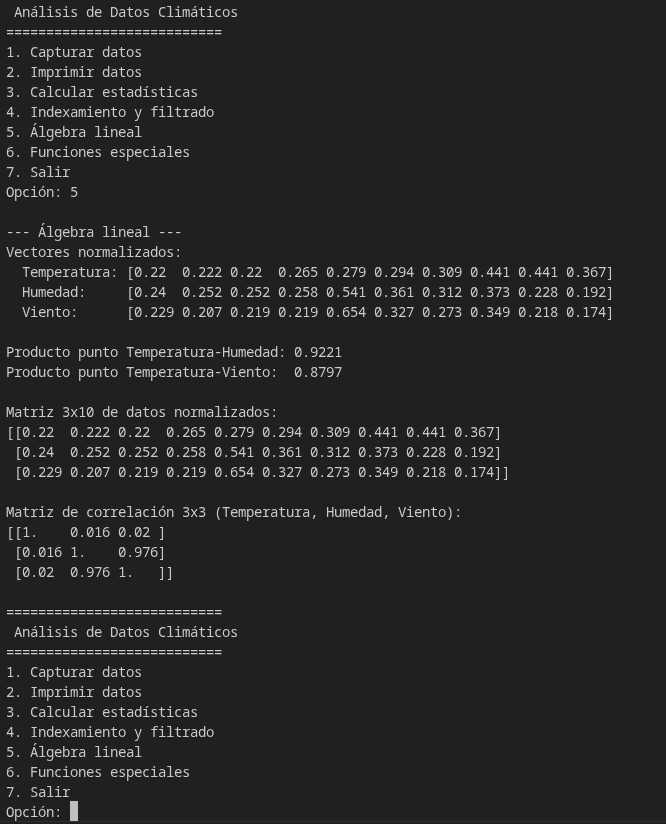
\includegraphics[width=0.5\textwidth]{Figuras/6}
		\caption{Cálculo de Álgebra Lineal.}
		\label{fig:6}
	\end{figure}
	\begin{figure}[htbp]
		\centering
		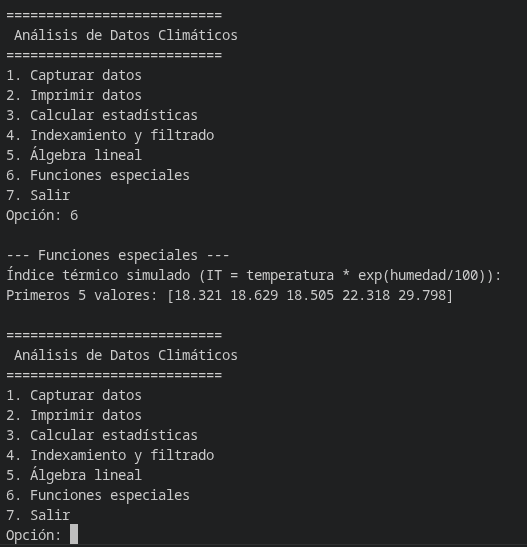
\includegraphics[width=0.5\textwidth]{Figuras/7}
		\caption{Funciones especiales}
		\label{fig:7}
	\end{figure}
	\begin{figure}[htbp]
		\centering
		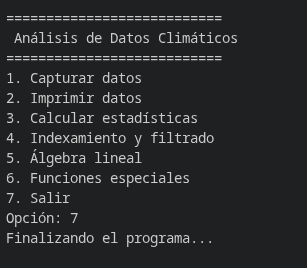
\includegraphics[width=0.5\textwidth]{Figuras/8}
		\caption{Salir del programa.}
		\label{fig:8}
	\end{figure}
	
	\section*{Conclusiones}
	La reusabilidad de funciones usadas en tareas anteriores contribuye a tener código reusable en todos los niveles.\\
	La carpeta en el repositorio de este proyecto es: \href{https://github.com/clivan/Programacion_y_Procesamiento_de_Datos_Infotec/2B}{Programación y procesamiento de Datos}.	
\end{document}
